\section{Muon / Tail Catcher Detector}
Most recent update: 2018-06-04 \\
Contact person: Valeri Saveliev (email : saveliev@mail.desy.de)

{\color{red} References not referred to in text}
%%%%%%%%%%%%%%%%%%%%%%%%%%%%%%%%%%%%%
\subsection{Introduction}
The main goals of the Muon System in the ILC Detector are the identification and reconstruction of the muons from inelastic $\Pep\Pem$ interactions over the largest possible energy and angular range and recover the energy leakage out of the hadron calorimeter (Energy Tail Catcher).
The physics goals set for the ILD detectors require that muons momentum are reconstructed with high precision of about $\Delta p_T/p^2_T = 2 \times10^{-5}$.
Due to the large amount of material muons have to traverse before reaching the muon detection system,  it cannot provide the required  momentum resolution and will be optimized mainly to the high efficiency and purity of muon identification.
A momentum resolution of this precision planned to be achieved with an excellent tracking system at ILC detector and important aspect is efficient linking of track candidates from the inner detectors with tracks in the muon detection system.
In addition to its muon identification ability, the first layers of the muon detection system will be optimized to act as a tail catcher for showers developing late in the calorimeters. This will improves the energy measurement in the hadron calorimeter, especially for the highest energy.
Another aspect of the muon system is the stand-alone identification and reconstruction of beam-halo muons. This requirement has an impact on the muon system granularity and time resolution, which shall be better than \unit[1]{ns}.

%%%%%%%%%%%%%%%%%%%%%%%%%%%%%%%%%%%%%%
\subsection{Conceptual Design of the Muon / Tail Catcher Detector}
Important constraints for the design of the muon system at ILC  as for many other experiments is the instrumentation of the detection elements inside the Iron return yoke, needed for the magnetic flux return of the detector solenoids.
The muon system/tail catcher detector instruments the Iron return yoke in the barrel and in the forward regions with maximal coverage.
The needed mechanical stability requires that the iron return yoke layer thickness is at least \unit[10]{cm}. The muon detectors will be interleaved between such Iron plates are used as muons absorber.
The requirement that the muon system/tail catcher serves both as a muon identification and as a tail catcher impacts its layout design.
The first section of the system provides ten relatively closely spaced layers, to act as a reasonable continuation of the hadron calorimeter.
As mentioned above the mechanical constraints limit between readout stations to be at least \unit[10]{cm}.
At the rear of the muon system the distance between stations can be much increased, since they only need to act as for the  muon identification and reconstruction.
Last three layers in the barrel, and two in the endcap are spaced \unit[60]{cm} apart.
The fact that the magnet coil adds about two interaction lengths of material in front of the muon detection system limits the effect of the tail catcher.
To maximize its impact the first sensitive layer is placed in front of the iron yoke, directly behind the coil and the first 10 layers are spaced more closely
to improve the calorimetric performance of the muon system.
Finally the yoke barrel part is equipped with one sensitive layer in front of the Iron yoke, 10 layers spaced \unit[14]{cm} apart, followed by three sensitive layers spaced by \unit[60]{cm} apart. The forward part of the yoke is equipped with 10 layers spaced by \unit[14]{cm}, followed by two sensitive layers spaced by \unit[60]{cm}. The overall layout of the muon system/tail catcher is shown in Figure~\ref{fig:ild:muon:concept}.
\begin{figure}
	\centering
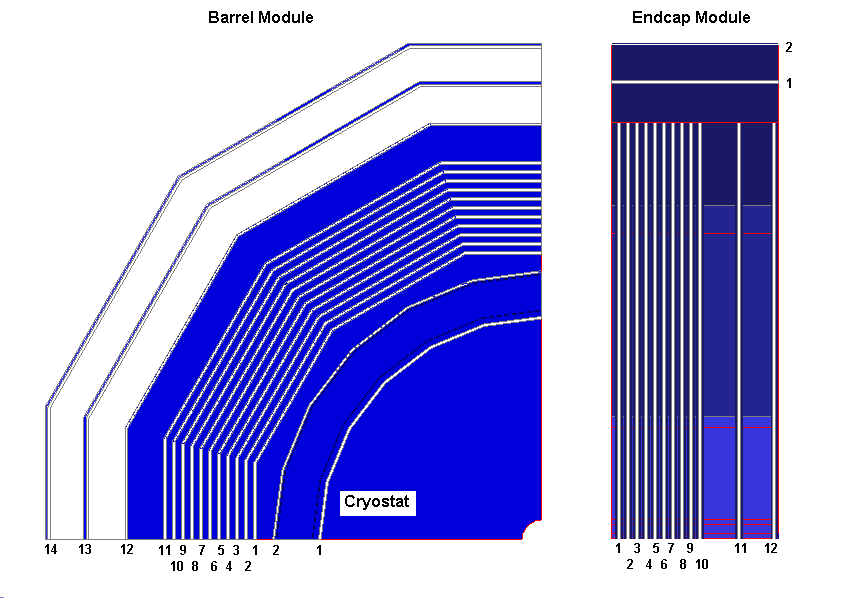
\includegraphics[height=8cm]{MuonDetector/MuonDetectorILD/2D_barel_endcap.png}
	\caption{Sensitive Layers of ILD Muon /Tail Catcher Detector}
	\label{fig:ild:muon:concept}
\end{figure}

Two main options are investigated for the muon detection elements: scintillator strips equipped with wave-length shifting fibers and readout with silicon photomultipliers (Sc/SiPM), or resistive plate chambers (RPC).

%%%%%%%%%%%%%%%%%%%%%%%%%%%%%%%%%%%%
\section{Scintillator/Silicon Photomultiplier}
Contact person: Valeri Saveliev (email : saveliev@mail.desy.de )

\subsection{Introduction}
The main option for the sensitive layers will use extruded plastic scintillation strips, composed of polystyrene doped with 1.0\% PPO and 0.03\% POPOP.
The extruded scintillator a width of $\unit[25-30]{mm}$ and thickness of \unit[7-10]{mm}.

A \unit[1]{mm} wide extruded groove running along the centre of the strip will take a commercially available wave length shifting (WLS) fibers.
The groove was filled with a white epoxy made of DER 332 resin and Jeffamine.

The scintillator strips will be covered on the outside by a layer of \ce{TiO2}, that is co-extruded alongside the scintillator during the extrusion process.

The maximal length of strips required for ILD is $\unit[200-250]{cm}$.

The signals will be readout from both sides of the strips by Silicon photomultipliers, coupled to the wave length shifting (WLS) fibres.
Reading out both sides of a strip offers the possibility to define the position of the hits along the strip, which will help in reducing the fake rate in the muon system.

Figure~\ref{fig:ild:muon:concept} (left) shows the design of the scintillator strip. The right picture presents the signal (number of photons) of the scintillation strip with WLS and SiPM readout from both sides.

\begin{figure}
	\centering
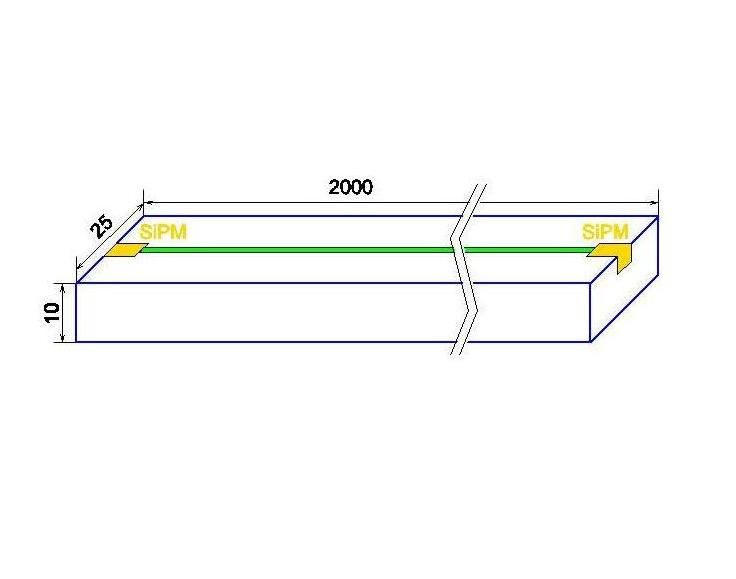
\includegraphics[height=8cm]{MuonDetector/MuonDetectorILD/Sc_strip.jpg}
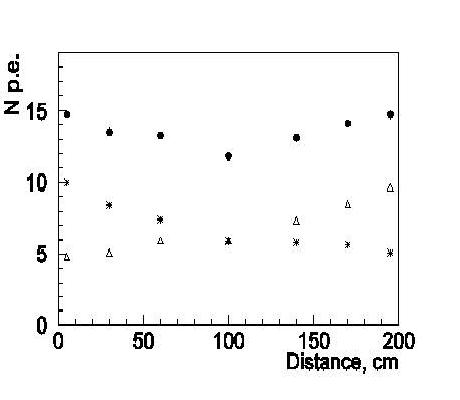
\includegraphics[height=8cm]{MuonDetector/MuonDetectorILD/Sc_strip_photons.jpg}
	\caption{Sensitive Layers of ILD Muon /Tail Catcher Detector and number of detected photons}
	\label{fig:ild:muon:concept}
\end{figure}

%%%%%%%%%%%%%%%%%%%%%%%%%%%%%%%%%%%%
\subsection{Recent Milestones}
The major R\&D effort of the Muon / Tail Catcher Development was concentrated on the optimization of the overall structure of the Muon System/ Tail Catcher:
\begin{enumerate}
\item Detailed Full Monte Carlo Simulation of the Muon System/Tail Catcher, it is concern to choose the geometry of detection plane, geometry of the stereo layers, number of the layers of the detection system and their position, especially concern to the energy leakage,
\item Study of the performance of the Muon System/Tail Catcher with framework of PFA,
\item Optimization of the detection elements of the Muon System/Tail Catcher. The first priority is the design of the main detection elements a scintillation strips with the SiPM readout,
\item Development of the Digital options of the SiPM for the Muon /Tail Catcher System, which will dramatically simplify the readout electronics and data processing.
\end{enumerate}

%%%%%%%%%%%%%%%%%%%%%%%%%%%%%%%%%%%%
\subsection{Engineering Challenges}
The main engineering challenge is the build the Distributed Large Scale of the Muon /Tail Catcher System and their embedment in the Solenoid Magnet Yoke.
Several layouts for the muon system have been tested.
This year will start the study of the integration of the large scale distributed Muon System/Tail Catcher Detectors in the Structure of the Solenoid Magnet Yoke.

\subsection{Future Plans}
Continue of the optimization of the Muon System/Tail Catcher on base detailed Monte Carlo Simulation and Reconstruction Chain,
\begin{itemize}
\item The performance of the muon system has been evaluated by simulating events in the ILD concept. To determine the optimal layout,
a geometry was created in MOKKA [3] with 19 layers in the barrel and 18 layers in the endcap, at equal distances of \unit[140]{mm}. After simulating the detector response
in  MOKKA once, different layouts could be studied by including or excluding layers in the reconstruction phase. For this study the muon layers have been segmented in pads of $30\times\unit[30]{mm^2}$.

\item Study of the Integration of the Muon System/Tail Catcher in to Solenoid Yoke,
\item Build of the prototypes of the Muon System/Tail Catcher detection elements on base of the Scintillator Strip/Wavelength Shifter and Analog SiPMs for the study of the main elements as thickness, length, reflection coating, wavelength shifters light yield and other. For this purposes will be develop the test setup for the cosmic muons detection,
\item Design and Technology development of the Analog SiPMs on base CMOS technology as preliminary options for the Muon System/Tail Catcher optimization,
\item Technology Development of the Digital option of the SiPMs on base innovative 3D interconnection (3D-IC) technology with fully digital readout and processing electronics.
\end{itemize}

\subsection{Applications Outside of Linear Colliders}
The development of the Digital SiPMs will have strong impact on the many application areas

One of the important application of practically full design and technology of the Muon /Tail Catcher System in the Homeland Security is the Muon Tomography for the security checking of the transport containers. The checking of the millions of the transport container in present time is one of the crucial and urgent problems, which don't have the efficient solution. The muon tomography, based on the HEP Muon System could be solution.

The development of the Digital SiPMs will have strong impact in Nuclear Medicine, in particular development of  Positron Emission Tomography (PET).  The new generation of the PET scanners will be developed on base of the All Digital SiPM Readout with more advanced performance.

%%%%%%%%%%%%%%%%%%%%%%%%%%%%%%%%%%%%%%%%%%%
\section{Resistive Plate Chamber }
Contact person: Valeri Saveliev (email : saveliev@mail.desy.de )

\subsection{Introduction}

Resistive plate chambers (RPC) are considered as an alternative sensitive elements for the Muon/Tail Catcher Detector.
Main features are excellent granularity up to $1\times\unit[1]{cm^2}$ pads and one threshold (1-bit), i.e. digital readout or semi-digital readout

Several types of RPCs have been successfully constructed and tested in the worldwide HEP community and within the ILC R\&D program~\cite{}.

Resistive Plate Chambers (RPCs) are likely technology choices for the SiD ILC hadron calorimeter (HCAL) and MUON systems due to their low cost.
RPCs have often been used as muon detectors (BaBar and BELLE). RPCs are inexpensive to build and can be easily constructed in a variety of shapes and sizes.

The major concern with RPCs has been their aging characteristics (BaBar was forced to replace its original RPCs and BELLE had startup problems).
Despite the significant progress made in recent years in RPC $R\&D$, a full understanding of all aging mechanisms has not been reached.
For example, the precise role of gas contaminants such as \ce{HF} (acid produced by the breakdown of the Freon used in RPC gases) in initiating of hot spot and increased current remains to be understood. A thorough understanding of the physics and chemistry of RPCs is needed if this technology is to be chosen for use in an ILC detectors.

Glass RPCs running in saturated avalanche mode are being considered for the HCAL. A large ($\unit[40]{m^2}$ of RPCs) prototype system is being proposed
for beam tests in FY08. The construction schedule for the prototypes is ambitious and leaves little time for further studies of possible aging effects or of alternative gas mixes. A smaller parallel effort could focus solely on these details and would broaden the US expertise in this potentially vital technology.

Recently an attractive alternative to glass has emerged from $R\&D$ for the BESIII muon system. The BESIII have developed Bakelite RPCs that have thin plastic films covering the inner Bakelite surfaces which eliminate the need for the traditional linseed oil coating. This new material has intrinsically lower noise than the Bakelite/melamine electrodes used in both the LHC and BABAR detectors. Over 1000 chambers were built and installed for BESIII. The bulk resistivity of the Bakelite can be adjusted to allow higher rate capability than glass. The BESIII chambers operate in streamer mode. Studies of these chambers in saturated avalanche mode while monitoring the humidity and HF content of the output gas may prove this design to have significantly superior aging properties than standard RPCs.

Development of the RPC readout is going in collaborate with the SLAC KPIX group~\cite{}.

The test prototypes of the KPIX front end data acquisition chip in the readout of RPCs operating in the saturated avalanche mode. The SLAC group will provide several KPIX chips for testing and aid in the design of a chip carrier that will mate to the ~\unit[3]{cm} wide pickup strips of the RPCs. Initial tests of the device with existing Bakelite RPC chambers will establish the compatibility and robustness of the present design with actual RPC signals. If successful, the tests will be extended to glass RPCs as used in the HCAL prototype and to chambers constructed from BESIII Bakelite.
A second study will examine the production and absorption of $F-(HF)$ in glass and BESIII RPCs and compare them to standard RPCs with linseed oil. Previous studies have found clear correlations between contaminants such as HF and increased noise rates and currents. Bakelite RPCs have been found to be sensitive to both the input gas and environmental humidity. A study of the humidity sensitivity of RPCs constructed from BESIII Bakelite will help determine the optimal operating conditions for these chambers.

%%%%%%%%%%%%%%%%%%%%%%%%%%%%%%%%%%%%%%%%%%%
\subsection{Future Plans}
\begin{enumerate}
\item Measure and predict the aging characteristics of the Bakelite RPCs to establish them as alternatives to standard glass or Bakelite RPCs,
\item Gain experience with glass RPCs while studying possible aging mechanisms. Study of alternative RPC gases could identify gas mixes that would minimize the production of harmful contaminants which lead to premature chamber aging,
\item Validate the use of the KPIX front-end chip for RPC readout.
\end{enumerate}


\begin{itemize}
	\item \fullcite{Repond:2010xh}
	\item \fullcite{1748-0221-7-04-P04015}
	\item \fullcite{Balagura2006590}
\end{itemize}
